\documentclass{article}

\usepackage{graphicx}
\usepackage{tikz}
\usepackage{tikzsymbols}
\usetikzlibrary{calc,patterns}
\usepackage{float}
\usepackage{pdflscape}
\usepackage{geometry}

\def\centerarc[#1](#2)(#3:#4:#5){\draw[#1] ($(#2)+({#5*cos(#3)},{#5*sin(#3)})$) arc (#3:#4:#5);}

\pagestyle{empty}
\begin{document}
    \centering
	\begin{figure}[H]
		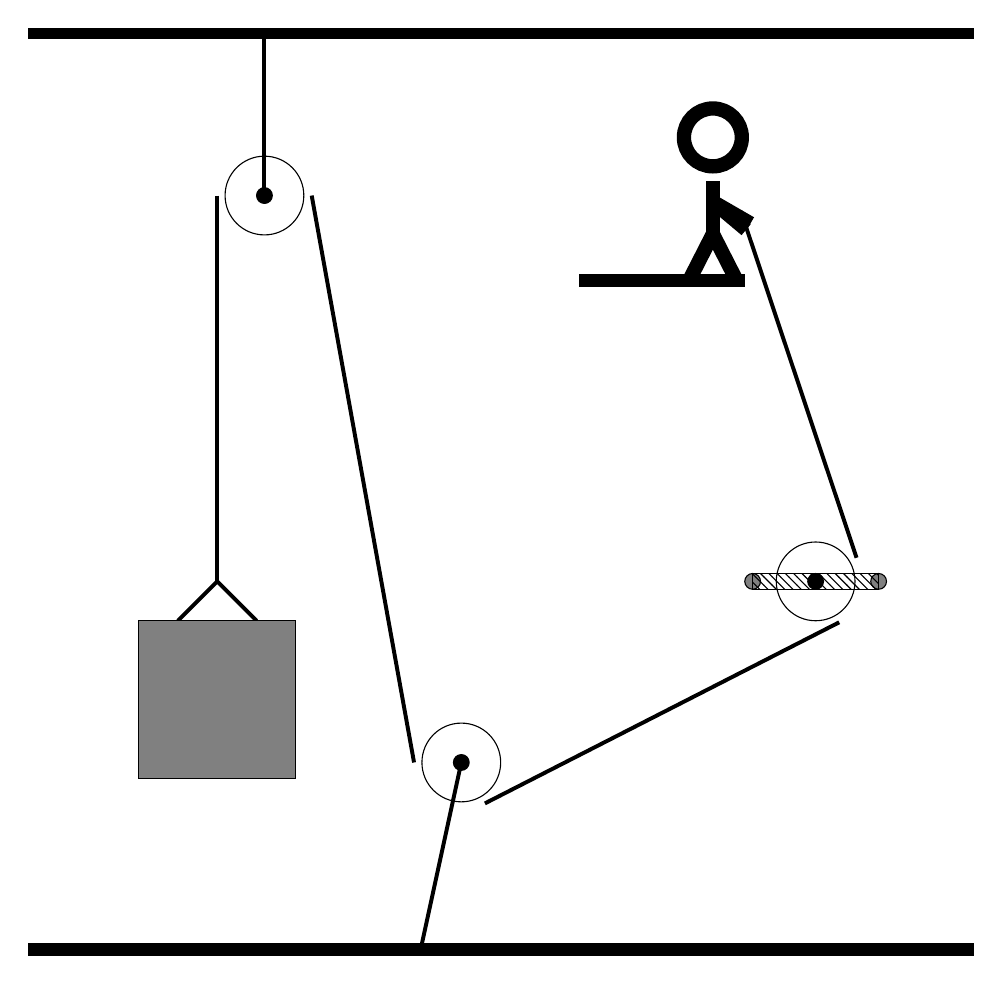
\begin{tikzpicture}
			%%%%% START %%%%%
			\def\a{11.5}
			\def\radlg{0.5}
			\def\radrp{0.6}
			\def\radsm{0.1}
			\def\yone{\a-2}
			\def\xone{1}
			\def\xtwo{3.5}
			\def\ytwo{\a-\a*0.8}
			\def\xthree{8}
			\def\ythree{\a-\a*0.6}
			\def\dx{6.75}
			\def\dy{\a-2}
			\def\hlena{\a*0.6}
			\def\width{0.5mm}
			\def\barbump{0.2}
			
			\draw[fill=black] (-2,\a) rectangle (10,\a+0.125);
					
			\draw (\xone,\yone) circle (\radlg);
			\draw[fill=black] (\xone,\yone) circle (\radsm);
			\draw[line width=\width] (\xone,\a) -- (\xone,\yone);
			
			\draw (\xtwo,\ytwo) circle (\radlg);
			\draw[fill=black] (\xtwo,\ytwo) circle (\radsm);
			\draw[line width=\width] (\xtwo,\ytwo) -- (\xtwo-0.5,0);
			
			\draw[fill=white](\xthree,\ythree) circle (\radlg);
			\draw[fill=black] (\xthree,\ythree) circle (\radsm);
			\draw[fill=black!50] (\xthree+\radrp+\barbump,\ythree) circle (\radsm);
			\draw[fill=black!50] (\xthree-\radrp-\barbump,\ythree) circle (\radsm);
			\draw[pattern=north west lines, pattern color=black] (\xthree-\radrp-\barbump,\ythree+0.1) rectangle (\xthree+\radrp+\barbump,\ythree-0.1); 
			
			\draw[line width=\width](\xone-0.5-\radrp,\a-\hlena-0.5) --  (\xone-\radrp,\a-\hlena) -- (\xone+0.5-\radrp,\a-\hlena-0.5);			
			\draw[fill=black!50] (\xone-1-\radrp,\a-\hlena-0.5) rectangle (\xone+1-\radrp,\a-\hlena-2-0.5); 
			
			\draw[line width=\width](\xone-\radrp,\yone) -- (\xone-\radrp,\a-\hlena);
			\centerarc[line width=\width](\xone,\yone)(180:0:\radrp)
			\draw[line width=\width](\xone+\radrp,\yone) -- (\xtwo-\radrp,\ytwo);
			\centerarc[line width=\width](\xtwo,\ytwo)(180:300:\radrp);
			\draw[line width=\width]({\xtwo+\radrp*cos(300)},{\ytwo+\radrp*sin(300)}) -- ({\xthree+\radrp*cos(300)},{\ythree+\radrp*sin(300)});
			\centerarc[line width=\width](\xthree,\ythree)(300:390:\radrp);
			\draw[line width=\width]({\xthree+\radrp*cos(390)},{\ythree+\radrp*sin(390)}) -- (\dx+0.3,\dy-0.2);

			\node at (\dx,\dy) {\Strichmaxerl[10][-220][-30]};
			\draw[fill=black] (5,\a-3) rectangle (7.1,\a-3.15);

			\draw[fill=black] (-2,0) rectangle (10,-0.15);
			%%%%% END %%%%%
		\end{tikzpicture}
	\end{figure}
\end{document}